\documentclass{article}%
\usepackage[T1]{fontenc}%
\usepackage[utf8]{inputenc}%
\usepackage{lmodern}%
\usepackage{textcomp}%
\usepackage{lastpage}%
\usepackage{geometry}%
\geometry{margin=0.5in,headheight=10pt,footskip=0.2in,tmargin=0.5in,bmargin=0.5in}%
\usepackage{graphicx}%
\usepackage{float}%
\usepackage{booktabs}%
\usepackage{hyperref}%
\usepackage{caption}%
\usepackage{subcaption}%
\usepackage{ragged2e}%
%
\title{ML Raport}%
\author{AutoPrep}%
\date{\today}%
%
\begin{document}%
\normalsize%
\maketitle%

    \begin{abstract}
    This raport has been generated with AutoPrep.
    \end{abstract}
    %
\tableofcontents%
\newpage%
\section{Overview}%
\label{sec:Overview}%

%
\subsection{System}%
\label{subsec:System}%

%


\begin{table}[H]%
\begin{center}%
\begin{tabular}{l l}%
\hline%
System&Windows\\%
Machine&AMD64\\%
Processor&Intel64 Family 6 Model 140 Stepping 2, GenuineIntel\\%
Architecture&64bit\\%
Python Version&3.11.5\\%
Physical Cores&4\\%
Logical Cores&8\\%
CPU Frequency (MHz)&1207.00\\%
Total RAM (GB)&15.74\\%
Available RAM (GB)&1.48\\%
Total Disk Space (GB)&457.28\\%
Free Disk Space (GB)&237.54\\%
\hline%
\end{tabular}%
\end{center}%
\caption{System overview.}%
\end{table}

%
\subsection{Dataset}%
\label{subsec:Dataset}%

%


\begin{table}[H]%
\begin{center}%
\begin{tabular}{l l}%
\hline%
Number of samples&1047\\%
Number of features&13\\%
Number of numerical features&6\\%
Number of categorical features&7\\%
\hline%
\end{tabular}%
\end{center}%
\caption{Dataset Summary.}%
\end{table}

%


\begin{table}[H]%
\begin{center}%
\begin{tabular}{l l l}%
\hline%
\textbf{class}&\textbf{number of observations}&\textbf{Percentage}\\%
\hline%
0&665&0.64\\%
1&382&0.36\\%
\hline%
\end{tabular}%
\end{center}%
\caption{Target class distribution.}%
\end{table}

%


\begin{table}[H]%
\begin{center}%
\begin{tabular}{l l l}%
\hline%
\textbf{classgit}&\textbf{number of observations}&\textbf{Percentage}\\%
\hline%
pclass&0&0.00\\%
name&0&0.00\\%
sex&0&0.00\\%
age&207&0.20\\%
sibsp&0&0.00\\%
parch&0&0.00\\%
ticket&0&0.00\\%
fare&1&0.00\\%
cabin&813&0.78\\%
embarked&1&0.00\\%
boat&672&0.64\\%
body&948&0.91\\%
home\_\_dest&453&0.43\\%
\hline%
\end{tabular}%
\end{center}%
\caption{Missing values distribution.}%
\end{table}

%


\begin{table}[H]%
\begin{center}%
\begin{tabular}{l l l l}%
\hline%
\textbf{class}&\textbf{type}&\textbf{dtype}&\textbf{space usage}\\%
\hline%
pclass&numerical&uint8&9.4 kB\\%
name&categorical&object&96.4 kB\\%
sex&categorical&category&9.7 kB\\%
age&numerical&float64&16.8 kB\\%
sibsp&numerical&uint8&9.4 kB\\%
parch&numerical&uint8&9.4 kB\\%
ticket&categorical&object&75.1 kB\\%
fare&numerical&float64&16.8 kB\\%
cabin&categorical&object&42.1 kB\\%
embarked&categorical&category&9.7 kB\\%
boat&categorical&object&46.4 kB\\%
body&numerical&float64&16.8 kB\\%
home\_\_dest&categorical&object&64.5 kB\\%
\hline%
\end{tabular}%
\end{center}%
\caption{Features dtypes description.}%
\end{table}

%


\begin{table}[H]%
\begin{center}%
\begin{tabular}{l l l l l l l l l}%
\hline%
\textbf{index}&\textbf{count}&\textbf{mean}&\textbf{std}&\textbf{min}&\textbf{25\%}&\textbf{50\%}&\textbf{75\%}&\textbf{max}\\%
\hline%
pclass&1047.00&2.30&0.84&1.00&2.00&3.00&3.00&3.00\\%
age&840.00&29.53&14.27&0.17&21.00&28.00&38.62&80.00\\%
sibsp&1047.00&0.52&1.05&0.00&0.00&0.00&1.00&8.00\\%
parch&1047.00&0.40&0.89&0.00&0.00&0.00&0.00&9.00\\%
fare&1046.00&33.55&51.81&0.00&7.92&14.50&31.27&512.33\\%
body&99.00&160.90&98.35&1.00&73.50&156.00&255.50&328.00\\%
\hline%
\end{tabular}%
\end{center}%
\caption{Numerical features description.}%
\end{table}

%


\begin{table}[H]%
\begin{center}%
\begin{tabular}{l l l l l}%
\hline%
\textbf{index}&\textbf{count}&\textbf{unique}&\textbf{top}&\textbf{freq}\\%
\hline%
name&1047&1046&Connolly, Miss. Kate&2\\%
ticket&1047&773&CA. 2343&9\\%
cabin&234&161&B57 B59 B63 B66&5\\%
boat&375&25&13&34\\%
home\_\_dest&594&317&New York, NY&50\\%
\hline%
\end{tabular}%
\end{center}%
\caption{Categorical features description.}%
\end{table}

%
\section{Eda}%
\label{sec:Eda}%

%
\subsection{Eda}%
\label{subsec:Eda}%

%


\begin{figure}[H]%
\centering%
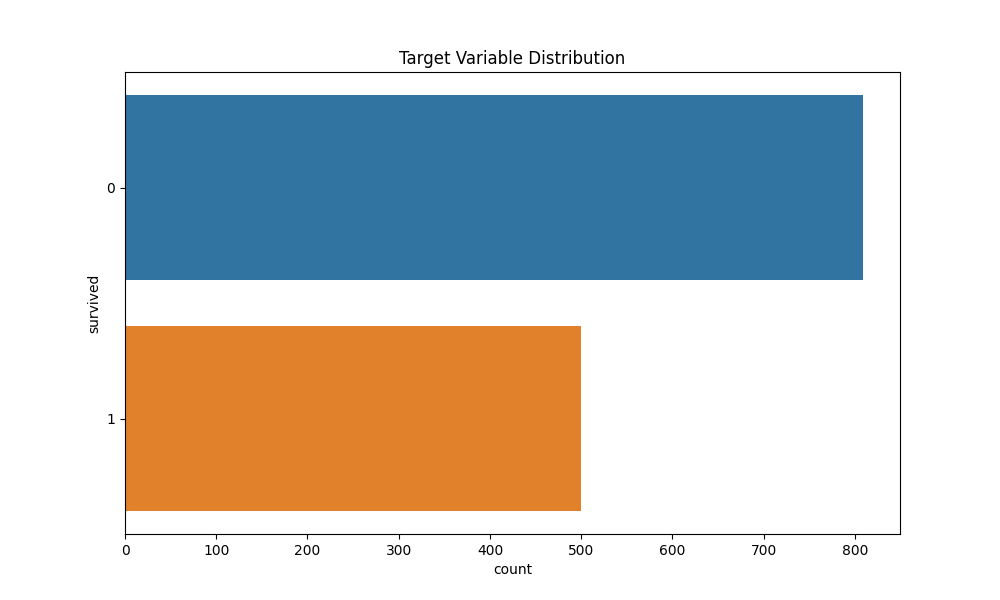
\includegraphics[width=0.9\textwidth]{C:/Users/rogal/MojGithub/AutoPrep/examples/raport/raport/charts/target_distribution.png}%
\caption{Target distribution.}%
\end{figure}

%


\begin{figure}[H]%
\centering%
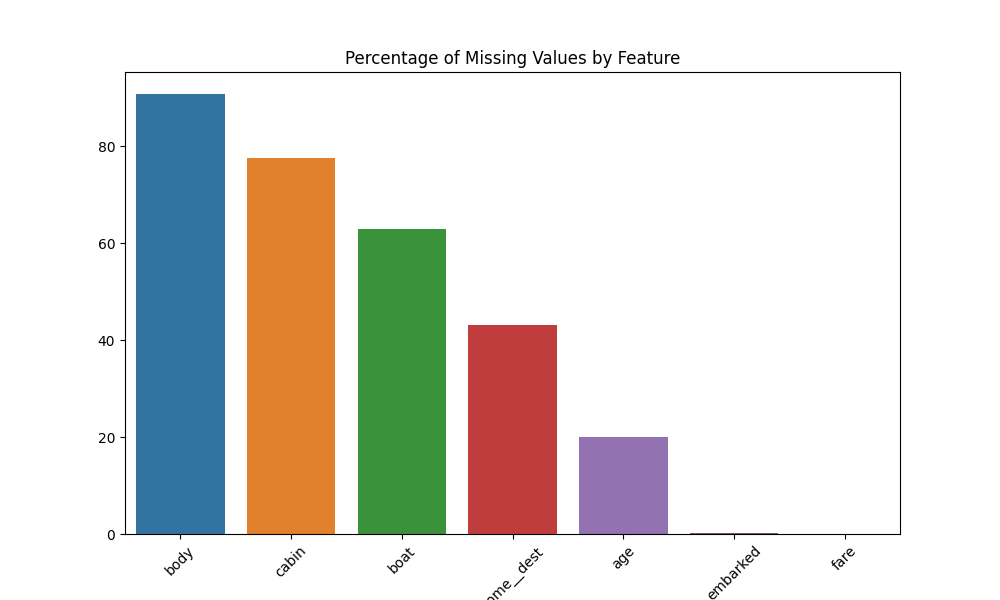
\includegraphics[width=0.9\textwidth]{C:/Users/rogal/MojGithub/AutoPrep/examples/raport/raport/charts/missing_values.png}%
\caption{Missing values.}%
\end{figure}

%
\subsection{Categorical}%
\label{subsec:Categorical}%

%


\begin{figure}[H]%
\centering%
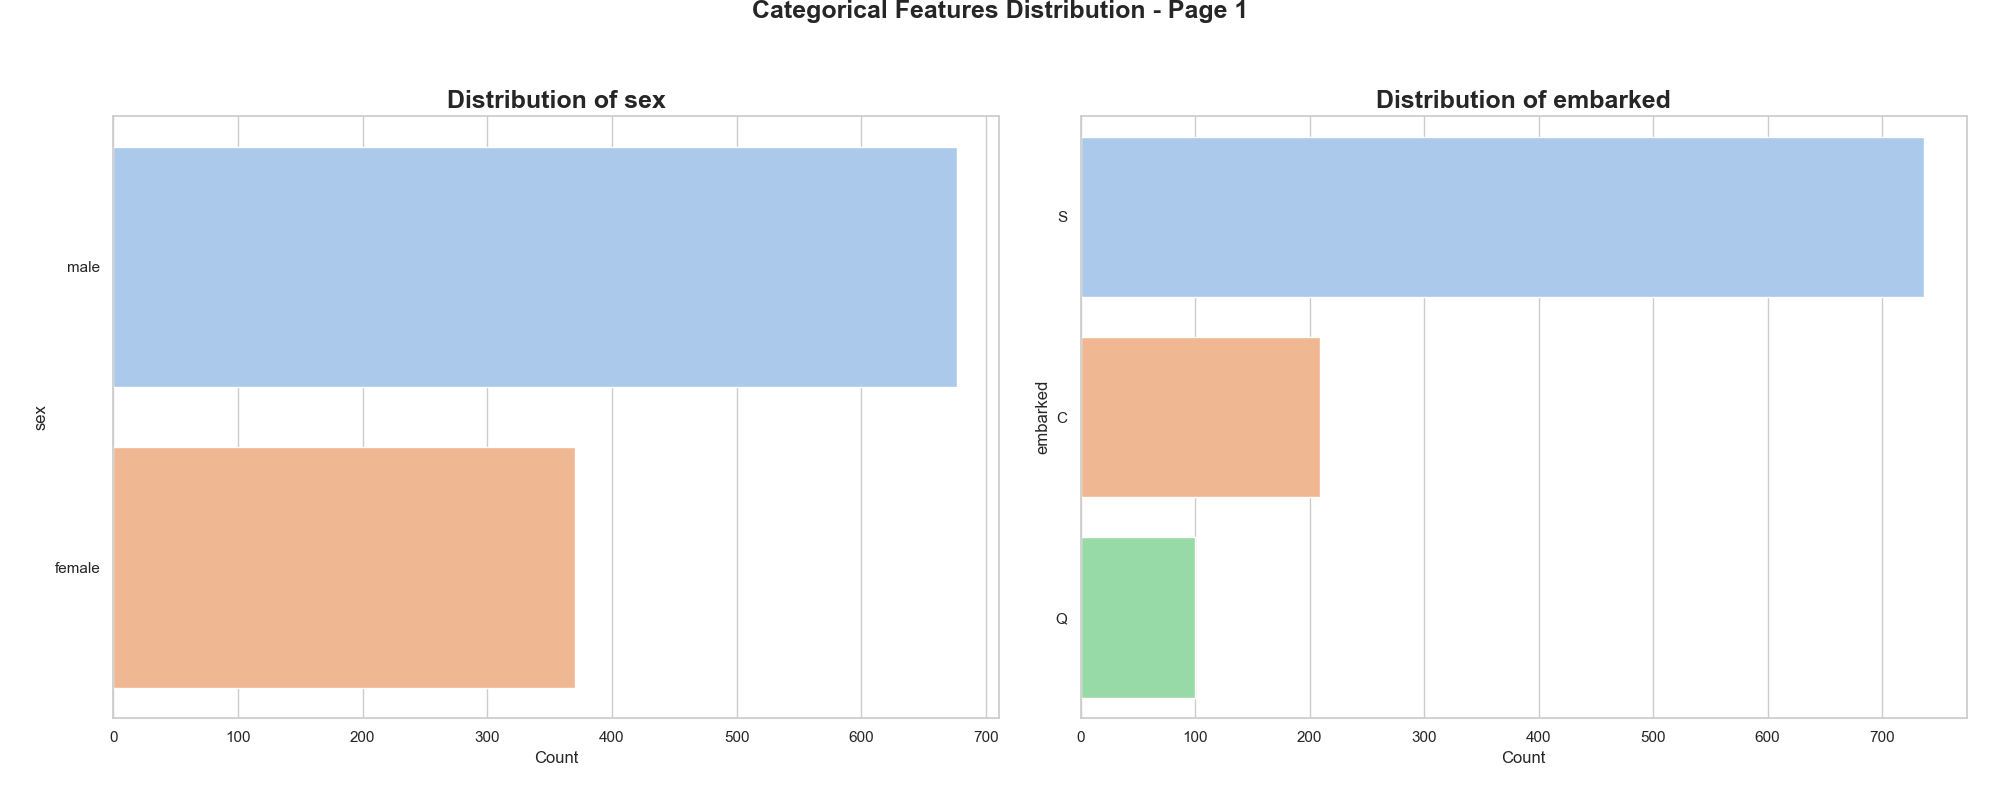
\includegraphics[width=0.9\textwidth]{C:/Users/rogal/MojGithub/AutoPrep/examples/raport/raport/charts/categorical_distribution_page_1.png}%
\caption{Categorical Features Distribution {-} Page 1}%
\end{figure}

%
\subsection{Numerical}%
\label{subsec:Numerical}%

%


\begin{figure}[H]%
\centering%
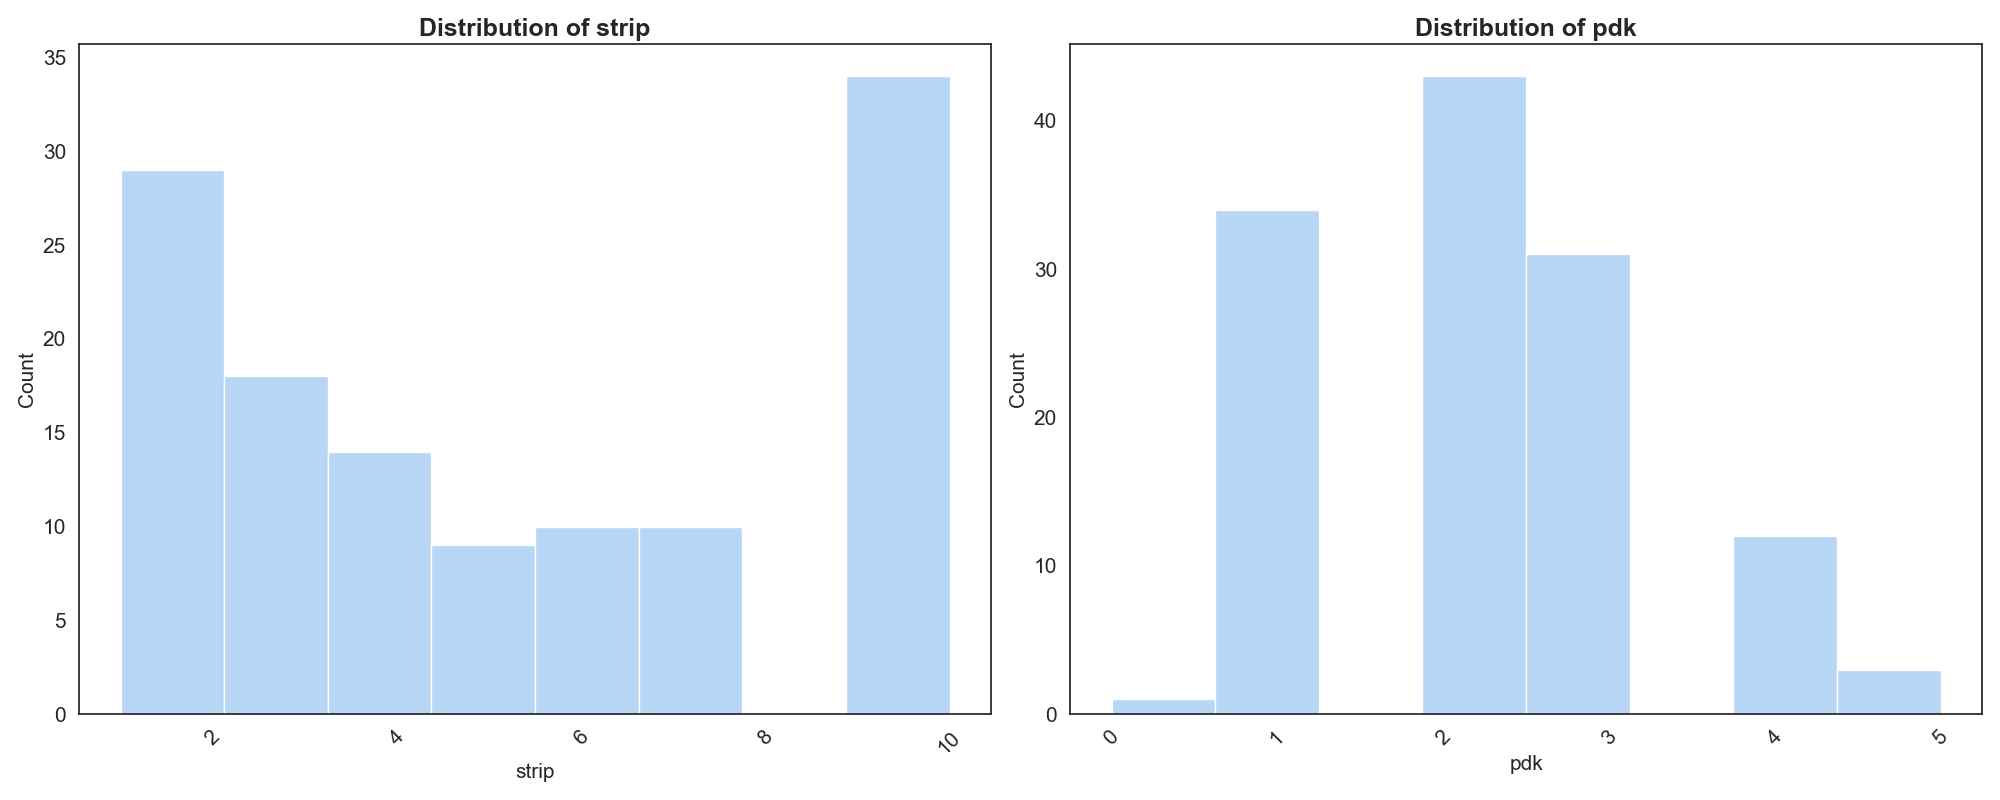
\includegraphics[width=0.9\textwidth]{C:/Users/rogal/MojGithub/AutoPrep/examples/raport/raport/charts/numerical_distribution_page_1.png}%
\caption{Numerical Features Distribution {-} Page 1}%
\end{figure}

%


\begin{figure}[H]%
\centering%
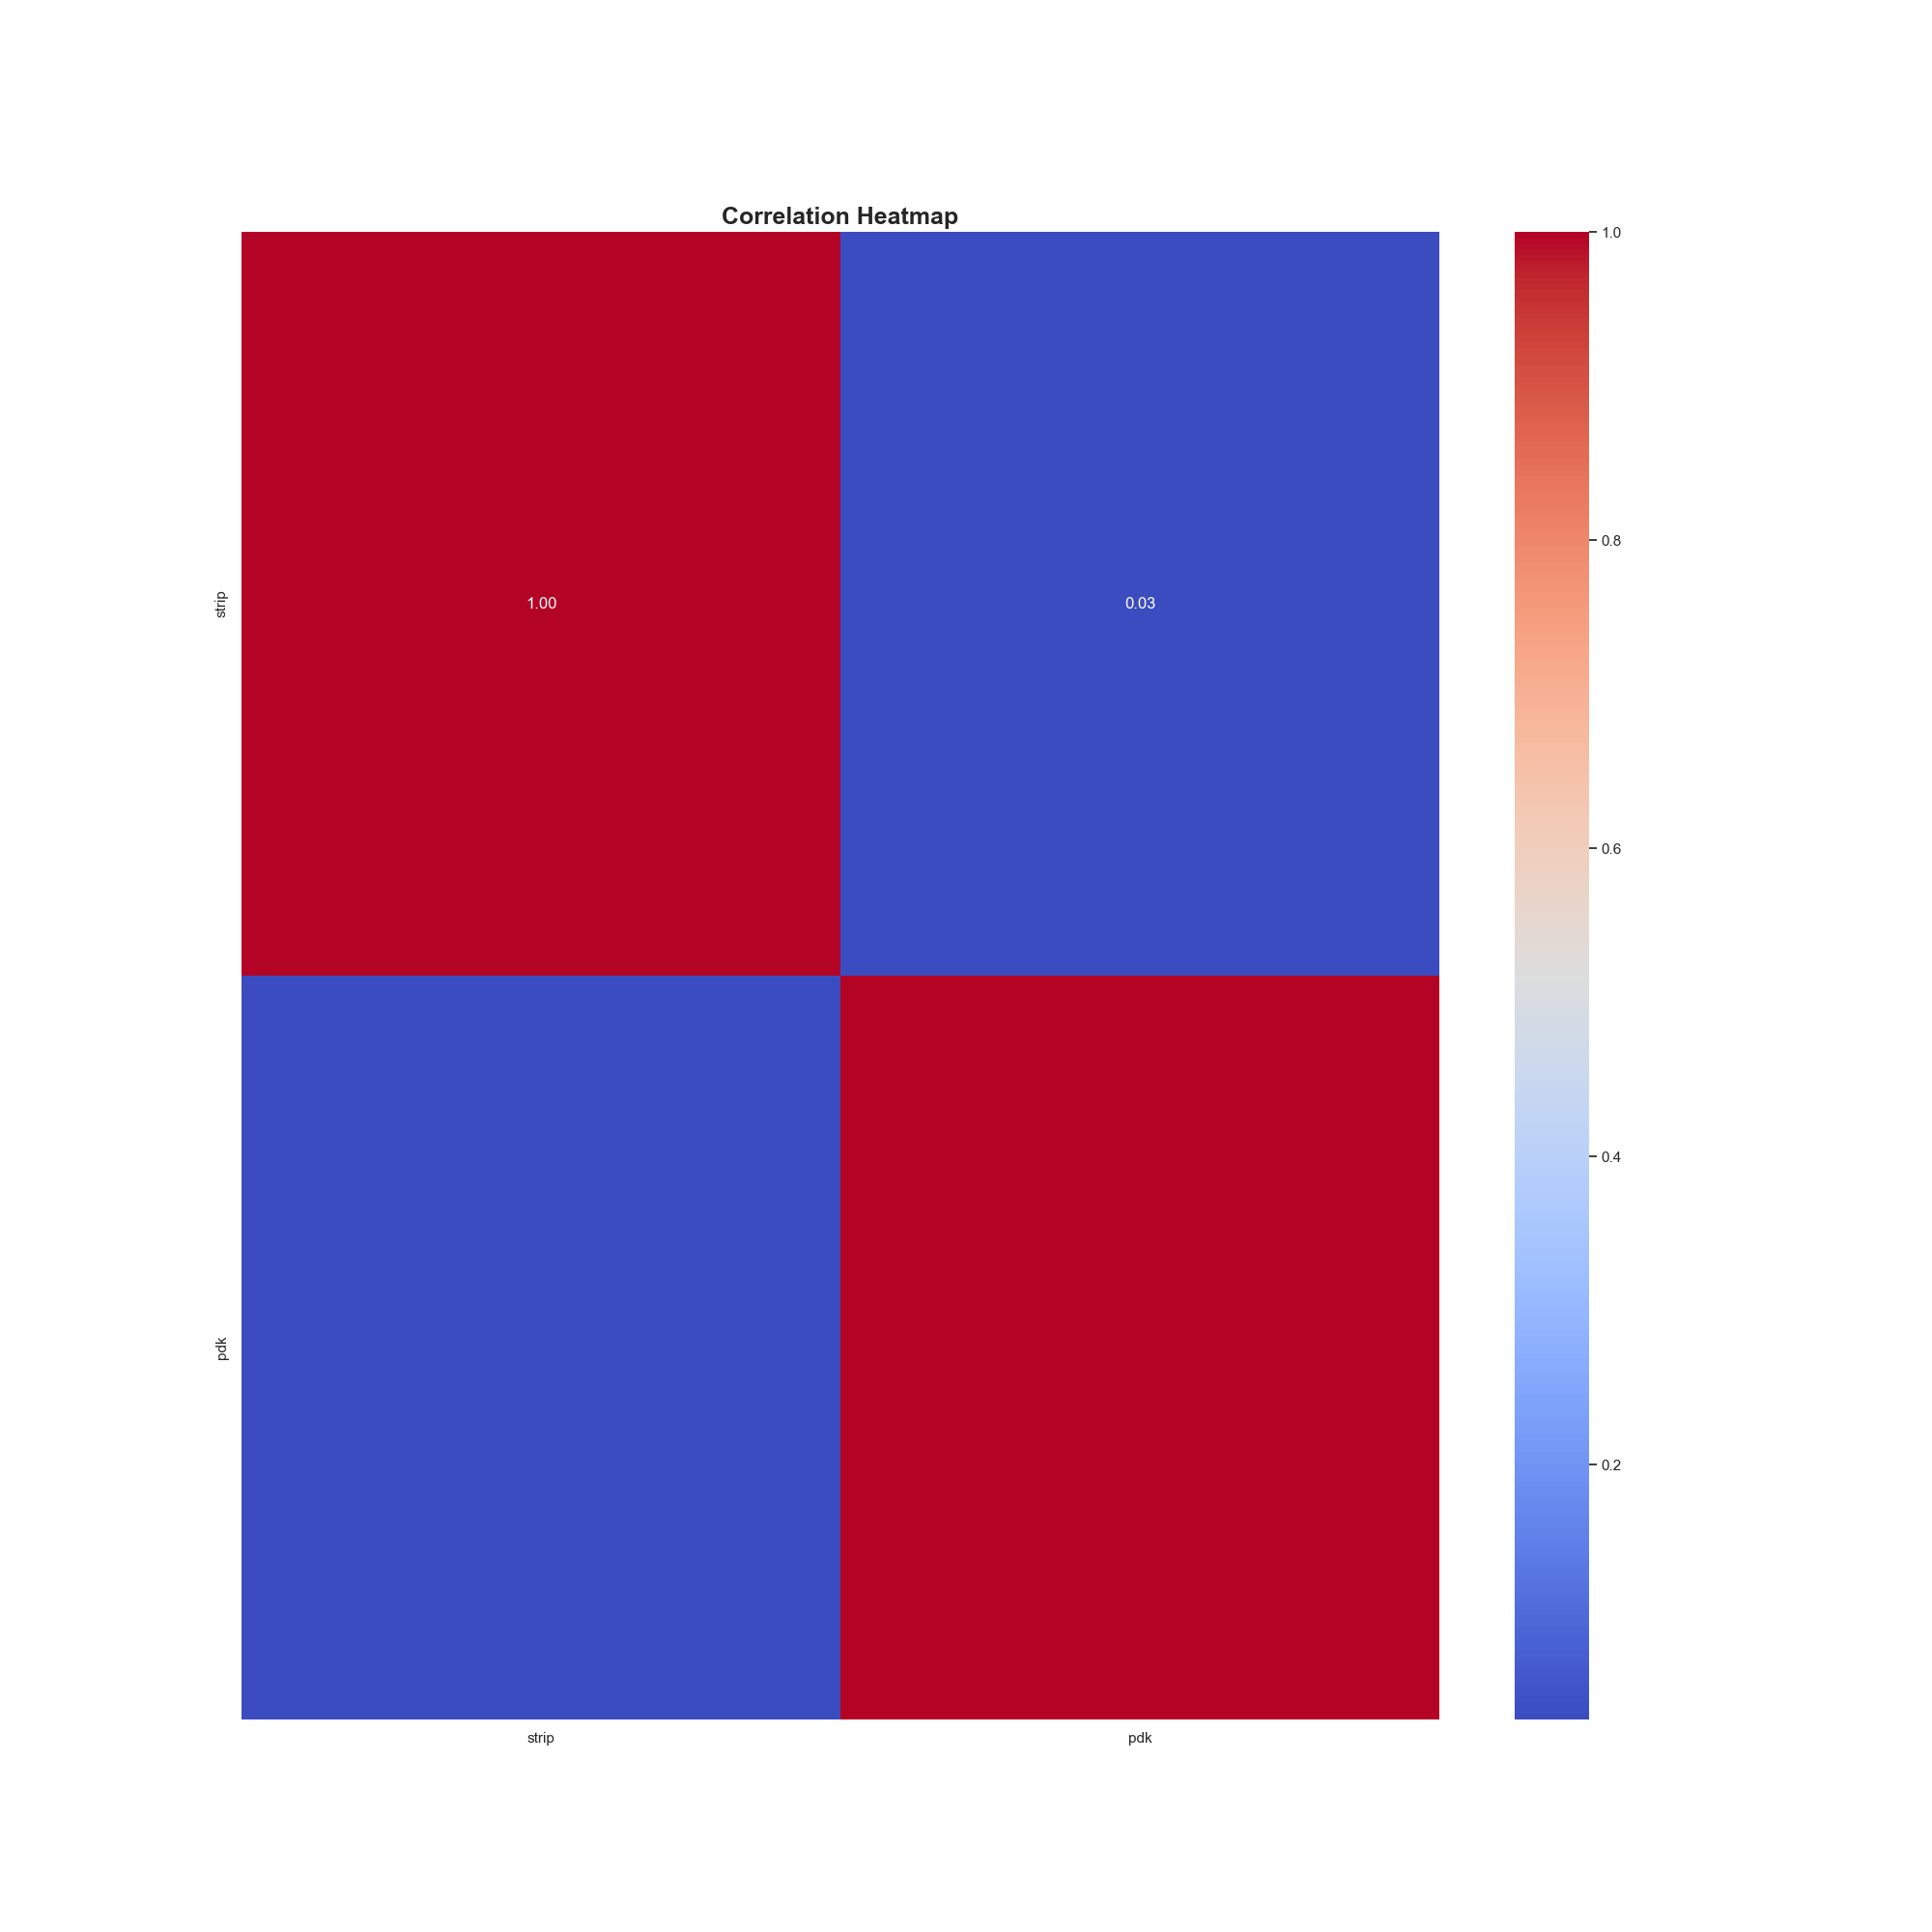
\includegraphics[width=0.9\textwidth]{C:/Users/rogal/MojGithub/AutoPrep/examples/raport/raport/charts/correlation_heatmap.png}%
\caption{Correlation heatmap.}%
\end{figure}

%


\begin{figure}[H]%
\centering%
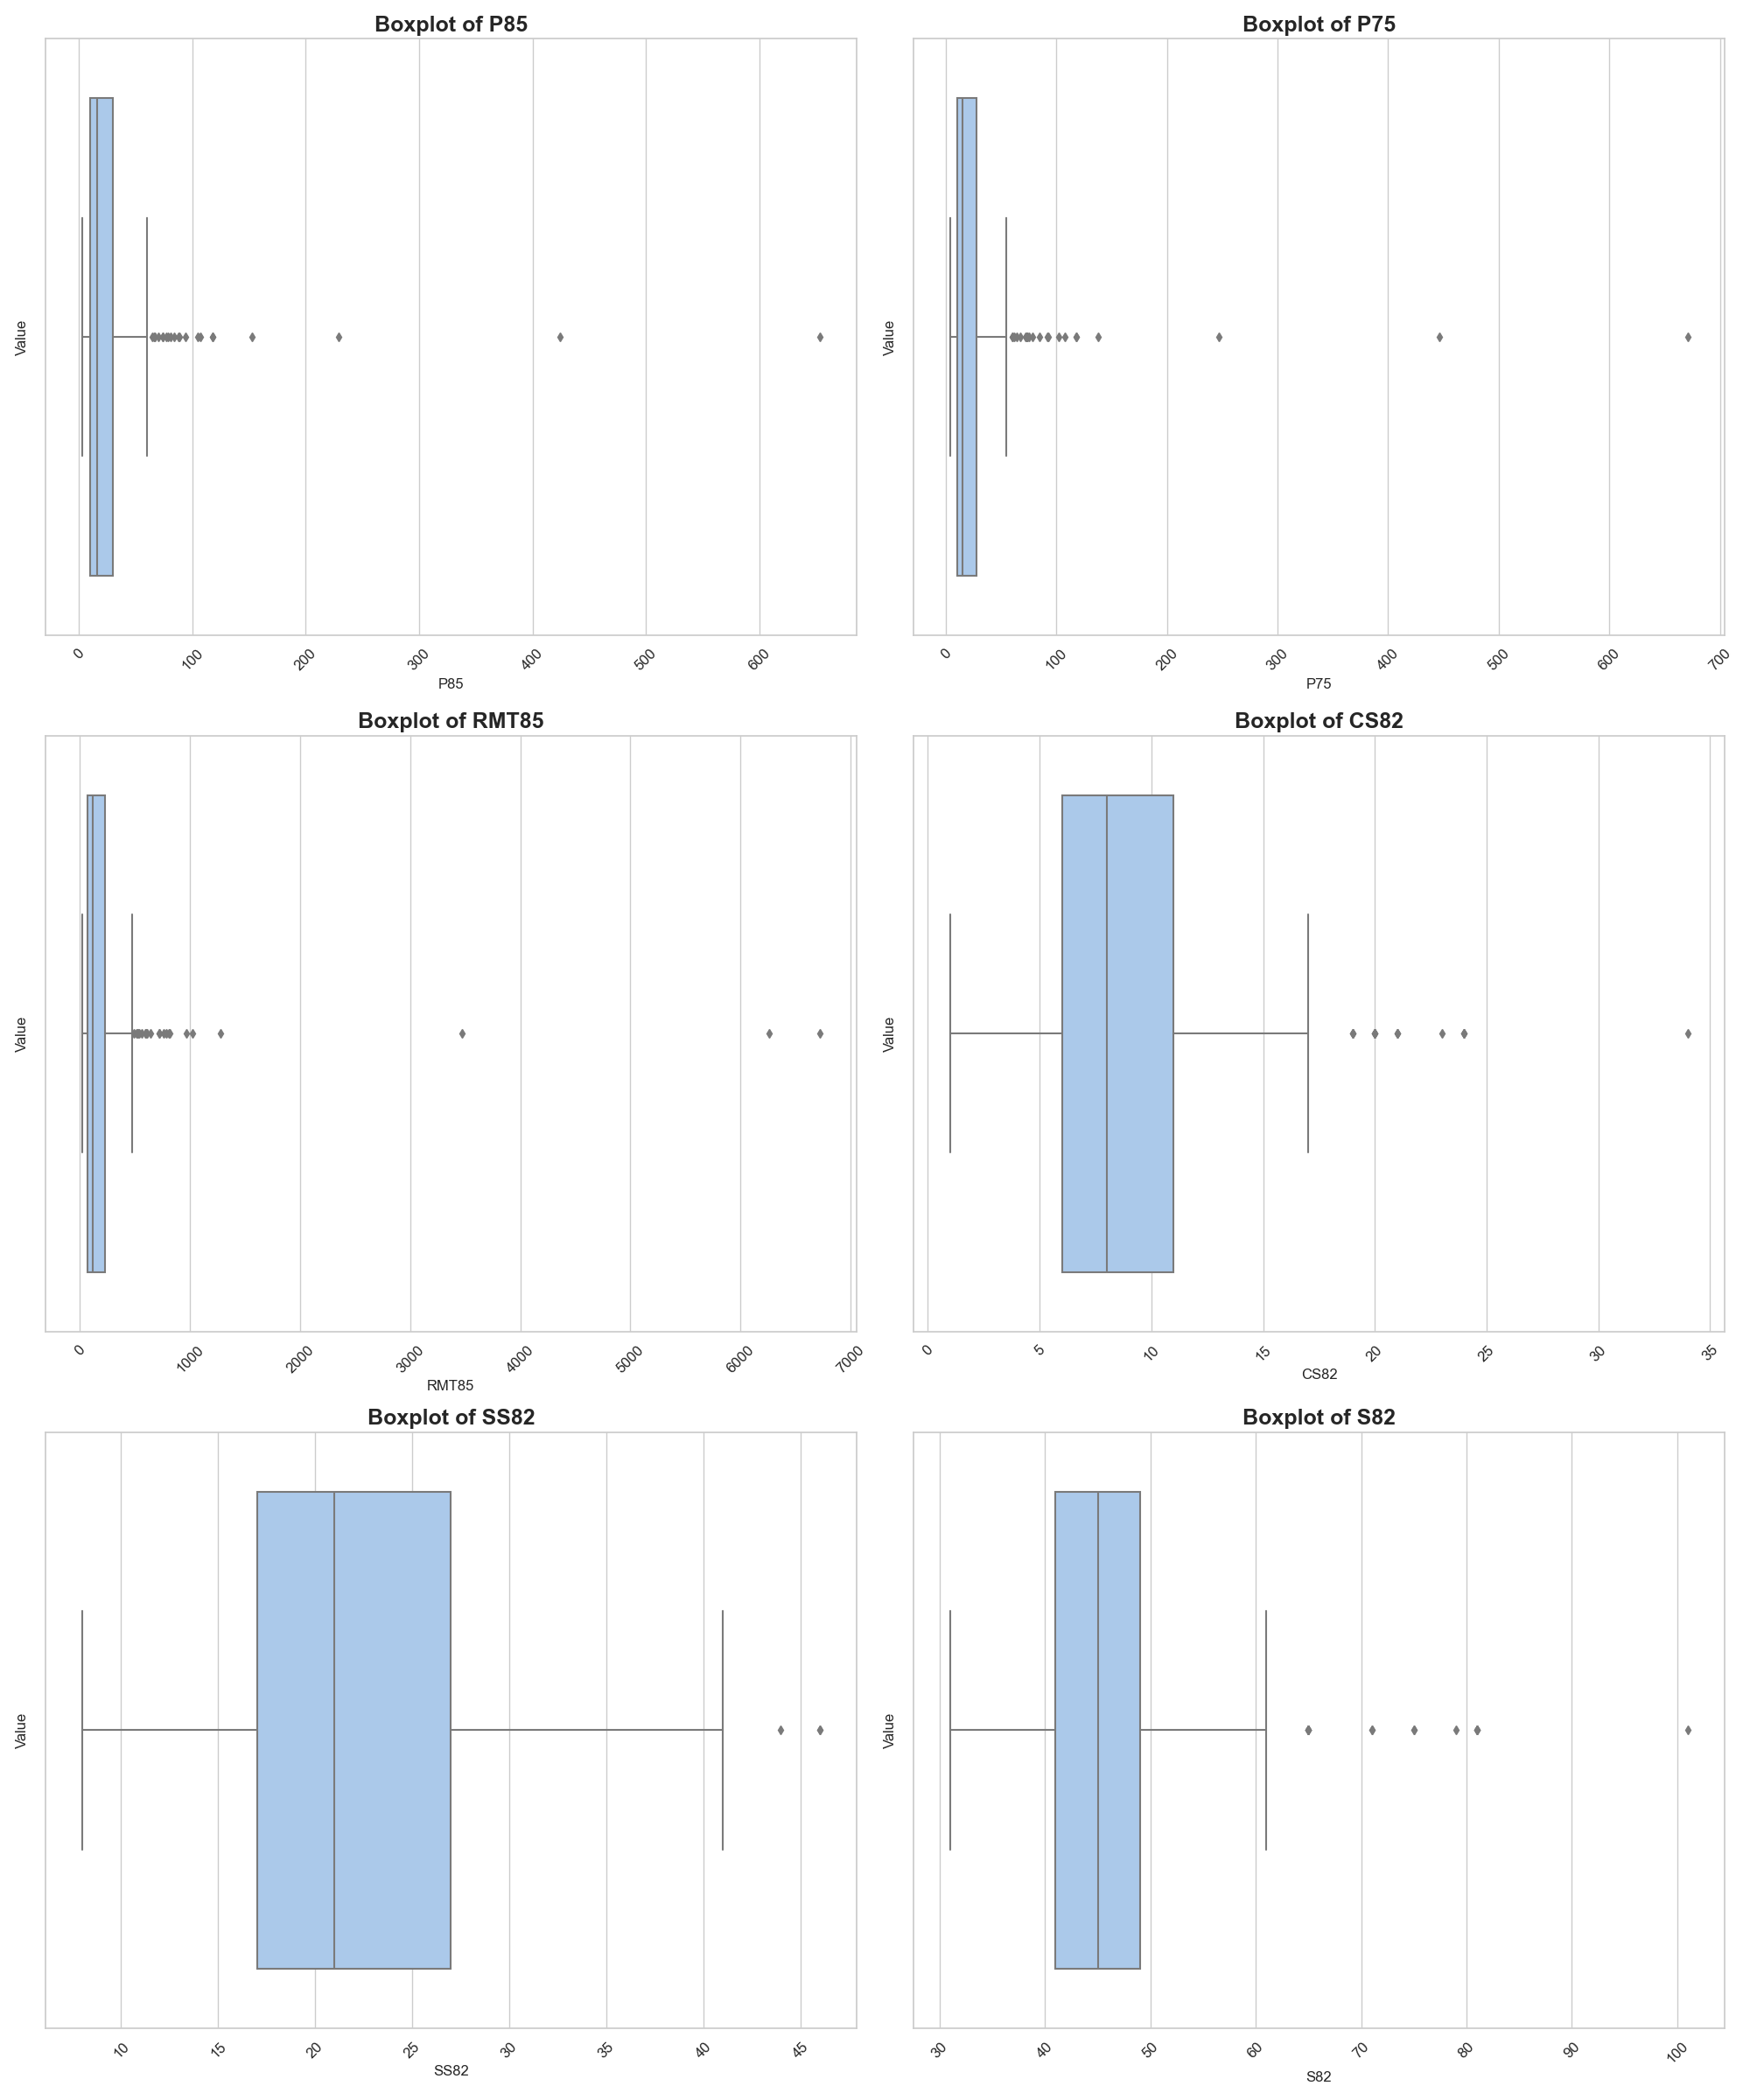
\includegraphics[width=0.9\textwidth]{C:/Users/rogal/MojGithub/AutoPrep/examples/raport/raport/charts/boxplot_page_1.png}%
\caption{Boxplot page 1}%
\end{figure}

%
\section{Preprocessing}%
\label{sec:Preprocessing}%

%


\begin{table}[H]%
\begin{center}%
\begin{tabular}{l l}%
\hline%
\textbf{Category}&\textbf{Value}\\%
\hline%
Unique created pipelines&2\\%
All created pipelines (after exploading each step params)&6\\%
All pipelines fit time&4 seconds\\%
All pipelines score time&5 seconds\\%
scores\_count&6.00\\%
scores\_mean&0.76\\%
scores\_std&0.01\\%
scores\_min&0.75\\%
scores\_25\%&0.75\\%
scores\_50\%&0.76\\%
scores\_75\%&0.77\\%
scores\_max&0.78\\%
Scoring function&<class 'str'>\\%
Scoring model&RandomForestClassifier\\%
\hline%
\end{tabular}%
\end{center}%
\caption{Preprocessing pipelines runtime statistics.}%
\end{table}

%


\begin{table}[H]%
\begin{center}%
\begin{tabular}{p{20mm} p{160mm}}%
\hline%
\textbf{index}&\textbf{steps}\\%
\hline%
0&NAImputer, UniqueFilter, ColumnEncoder, ColumnScaler, CorrelationFilter\\%
1&NAImputer, UniqueFilter, ColumnEncoder, ColumnScaler, VarianceFilter\\%
\hline%
\end{tabular}%
\end{center}%
\caption{Pipelines steps overview.}%
\end{table}

%


\begin{table}[H]%
\begin{center}%
\begin{tabular}{l l l l l}%
\hline%
\textbf{score index}&\textbf{file name}&\textbf{score}&\textbf{fit duration}&\textbf{score duration}\\%
\hline%
0&preprocessing\_pipeline\_0.joblib&0.78&a moment&a moment\\%
1&preprocessing\_pipeline\_1.joblib&0.77&a moment&a moment\\%
2&preprocessing\_pipeline\_2.joblib&0.77&a moment&a moment\\%
\hline%
\end{tabular}%
\end{center}%
\caption{Best preprocessing pipelines.}%
\end{table}

%


\begin{table}[H]%
\begin{center}%
\begin{tabular}{p{10mm} p{30mm} p{60mm} p{60mm}}%
\hline%
\textbf{step}&\textbf{name}&\textbf{description}&\textbf{params}\\%
\hline%
0&NAImputer&Imputes missing data.&\{"numeric\_imputer": "median", "categorical\_imputer": "most\_frequent"\}\\%
1&UniqueFilter&Removes categorical columns with 100\% unique values. Dropped columns: {[}{]}&\{\}\\%
2&ColumnEncoder&Encodes categorical columns using OneHotEncoder (for columns with <5 unique values) or TolerantLabelEncoder (for columns with >=5 unique values). Encodes target variable using LabelEncoder if provided.&\{\}\\%
3&ColumnScaler&Scales numerical columns using one of 3 scaling methods.&\{"method": "robust"\}\\%
4&VarianceFilter&Removes columns with zero variance. Dropped columns: {[}{]}&\{\}\\%
\hline%
\end{tabular}%
\end{center}%
\caption{0th best pipeline overwiev on training set.}%
\end{table}

%


\begin{table}[H]%
\begin{center}%
\begin{tabular}{l l l l l l l l l}%
\hline%
\textbf{index}&\textbf{count}&\textbf{mean}&\textbf{std}&\textbf{min}&\textbf{25\%}&\textbf{50\%}&\textbf{75\%}&\textbf{max}\\%
\hline%
pclass&1047.00&0.00&1.00&{-}1.55&{-}0.36&0.84&0.84&0.84\\%
name&1047.00&0.00&1.00&{-}1.73&{-}0.87&{-}0.00&0.87&1.73\\%
age&1047.00&{-}0.00&1.00&{-}2.27&{-}0.57&{-}0.10&0.45&3.97\\%
sibsp&1047.00&{-}0.00&1.00&{-}0.50&{-}0.50&{-}0.50&0.46&7.13\\%
parch&1047.00&0.00&1.00&{-}0.44&{-}0.44&{-}0.44&{-}0.44&9.63\\%
ticket&1047.00&{-}0.00&1.00&{-}1.68&{-}0.90&0.00&0.93&1.67\\%
fare&1047.00&0.00&1.00&{-}0.65&{-}0.49&{-}0.37&{-}0.04&9.25\\%
home\_\_dest&1047.00&{-}0.00&1.00&{-}2.72&{-}0.18&0.23&0.30&2.01\\%
sex\_female&1047.00&0.00&1.00&{-}0.74&{-}0.74&{-}0.74&1.35&1.35\\%
embarked\_C&1047.00&{-}0.00&1.00&{-}0.50&{-}0.50&{-}0.50&{-}0.50&2.00\\%
embarked\_Q&1047.00&0.00&1.00&{-}0.32&{-}0.32&{-}0.32&{-}0.32&3.08\\%
embarked\_S&1047.00&{-}0.00&1.00&{-}1.55&{-}1.55&0.65&0.65&0.65\\%
\hline%
\end{tabular}%
\end{center}%
\caption{0th best pipeline output overview.}%
\end{table}

%


\begin{table}[H]%
\begin{center}%
\begin{tabular}{p{10mm} p{30mm} p{60mm} p{60mm}}%
\hline%
\textbf{step}&\textbf{name}&\textbf{description}&\textbf{params}\\%
\hline%
0&NAImputer&Imputes missing data.&\{"numeric\_imputer": "median", "categorical\_imputer": "most\_frequent"\}\\%
1&UniqueFilter&Removes categorical columns with 100\% unique values. Dropped columns: {[}{]}&\{\}\\%
2&ColumnEncoder&Encodes categorical columns using OneHotEncoder (for columns with <5 unique values) or TolerantLabelEncoder (for columns with >=5 unique values). Encodes target variable using LabelEncoder if provided.&\{\}\\%
3&ColumnScaler&Scales numerical columns using one of 3 scaling methods.&\{"method": "standard"\}\\%
4&VarianceFilter&Removes columns with zero variance. Dropped columns: {[}{]}&\{\}\\%
\hline%
\end{tabular}%
\end{center}%
\caption{1th best pipeline overwiev on training set.}%
\end{table}

%


\begin{table}[H]%
\begin{center}%
\begin{tabular}{l l l l l l l l l}%
\hline%
\textbf{index}&\textbf{count}&\textbf{mean}&\textbf{std}&\textbf{min}&\textbf{25\%}&\textbf{50\%}&\textbf{75\%}&\textbf{max}\\%
\hline%
pclass&1047.00&0.65&0.42&0.00&0.50&1.00&1.00&1.00\\%
name&1047.00&0.50&0.29&0.00&0.25&0.50&0.75&1.00\\%
age&1047.00&0.36&0.16&0.00&0.27&0.35&0.44&1.00\\%
sibsp&1047.00&0.07&0.13&0.00&0.00&0.00&0.12&1.00\\%
parch&1047.00&0.04&0.10&0.00&0.00&0.00&0.00&1.00\\%
ticket&1047.00&0.50&0.30&0.00&0.23&0.50&0.78&1.00\\%
fare&1047.00&0.07&0.10&0.00&0.02&0.03&0.06&1.00\\%
home\_\_dest&1047.00&0.58&0.21&0.00&0.54&0.62&0.64&1.00\\%
sex\_female&1047.00&0.35&0.48&0.00&0.00&0.00&1.00&1.00\\%
embarked\_C&1047.00&0.20&0.40&0.00&0.00&0.00&0.00&1.00\\%
embarked\_Q&1047.00&0.10&0.29&0.00&0.00&0.00&0.00&1.00\\%
embarked\_S&1047.00&0.70&0.46&0.00&0.00&1.00&1.00&1.00\\%
\hline%
\end{tabular}%
\end{center}%
\caption{1th best pipeline output overview.}%
\end{table}

%


\begin{table}[H]%
\begin{center}%
\begin{tabular}{p{10mm} p{30mm} p{60mm} p{60mm}}%
\hline%
\textbf{step}&\textbf{name}&\textbf{description}&\textbf{params}\\%
\hline%
0&NAImputer&Imputes missing data.&\{"numeric\_imputer": "median", "categorical\_imputer": "most\_frequent"\}\\%
1&UniqueFilter&Removes categorical columns with 100\% unique values. Dropped columns: {[}{]}&\{\}\\%
2&ColumnEncoder&Encodes categorical columns using OneHotEncoder (for columns with <5 unique values) or TolerantLabelEncoder (for columns with >=5 unique values). Encodes target variable using LabelEncoder if provided.&\{\}\\%
3&ColumnScaler&Scales numerical columns using one of 3 scaling methods.&\{"method": "minmax"\}\\%
4&VarianceFilter&Removes columns with zero variance. Dropped columns: {[}{]}&\{\}\\%
\hline%
\end{tabular}%
\end{center}%
\caption{2th best pipeline overwiev on training set.}%
\end{table}

%


\begin{table}[H]%
\begin{center}%
\begin{tabular}{l l l l l l l l l}%
\hline%
\textbf{index}&\textbf{count}&\textbf{mean}&\textbf{std}&\textbf{min}&\textbf{25\%}&\textbf{50\%}&\textbf{75\%}&\textbf{max}\\%
\hline%
pclass&1047.00&{-}0.70&0.84&{-}2.00&{-}1.00&0.00&0.00&0.00\\%
name&1047.00&0.00&0.58&{-}1.00&{-}0.50&0.00&0.50&1.00\\%
age&1047.00&0.09&0.98&{-}2.14&{-}0.46&0.00&0.54&4.00\\%
sibsp&1047.00&0.52&1.05&0.00&0.00&0.00&1.00&8.00\\%
parch&1047.00&0.40&0.89&0.00&0.00&0.00&0.00&9.00\\%
ticket&1047.00&{-}0.00&0.55&{-}0.92&{-}0.49&0.00&0.51&0.91\\%
fare&1047.00&0.81&2.22&{-}0.62&{-}0.28&0.00&0.72&21.32\\%
home\_\_dest&1047.00&{-}0.48&2.06&{-}6.09&{-}0.86&0.00&0.14&3.66\\%
sex\_female&1047.00&0.35&0.48&0.00&0.00&0.00&1.00&1.00\\%
embarked\_C&1047.00&0.20&0.40&0.00&0.00&0.00&0.00&1.00\\%
embarked\_Q&1047.00&0.10&0.29&0.00&0.00&0.00&0.00&1.00\\%
embarked\_S&1047.00&{-}0.30&0.46&{-}1.00&{-}1.00&0.00&0.00&0.00\\%
\hline%
\end{tabular}%
\end{center}%
\caption{2th best pipeline output overview.}%
\end{table}

%
\section{Modeling}%
\label{sec:Modeling}%

%
\subsection{Overview}%
\label{subsec:Overview}%

%
This part of the report presents the results of the modeling process. There were 6 classification models trained and 3 of them selected based on the ROC AUC score.%
\newline%
\text{Models used in the modeling process}%
\newline%
\begin{itemize}%
\item%
DecisionTreeClassifier%
\item%
GaussianNaiveClassifier%
\item%
KNeighboursClassifier%
\item%
Logistic Regression%
\item%
SVC%
\item%
XGBoost%
\end{itemize}%
The table below presents the results of the modeling process on default parameters for each of the best piplelines. The models are sorted by the ROC AUC score in descending order.%


\begin{table}[H]%
\begin{center}%
\begin{tabular}{p{30mm} p{20mm} p{50mm}}%
\hline%
\textbf{Model}&\textbf{AUC Score}&\textbf{Pipeline}\\%
\hline%
SVC&0.77&preprocessing\_pipeline\_0\\%
XGBoost&0.77&preprocessing\_pipeline\_2\\%
XGBoost&0.77&preprocessing\_pipeline\_1\\%
\hline%
\end{tabular}%
\end{center}%
\caption{Results of the modeling process on default parameters}%
\end{table}

%
\subsection{Hyperparameter tuning}%
\label{subsec:Hyperparametertuning}%

%
This section presents the results of the hyperparameter tuning process for the best 3 models using RandomizedSearchCV.%
The following parameters grids were used for hyperparameter tuning:%


\begin{table}[H]%
\begin{center}%
\begin{tabular}{p{30mm} p{70mm}}%
\hline%
\textbf{Parameter}&\textbf{Values}\\%
\hline%
C&{[}0.1, 1, 10, 100, 1000{]}\\%
kernel&{[}'linear', 'poly', 'rbf', 'sigmoid'{]}\\%
degree&{[}3, 4, 5{]}\\%
gamma&{[}'scale', 'auto'{]}\\%
random\_state&{[}42{]}\\%
\hline%
\end{tabular}%
\end{center}%
\caption{Parameter grid for SVC}%
\end{table}

%


\begin{table}[H]%
\begin{center}%
\begin{tabular}{p{30mm} p{70mm}}%
\hline%
\textbf{Parameter}&\textbf{Values}\\%
\hline%
max\_depth&{[}3, 6, 7{]}\\%
learning\_rate&{[}0.01, 0.1, 0.3{]}\\%
subsample&{[}0.5, 0.8, 1.0{]}\\%
colsample\_bytree&{[}0.8, 1.0{]}\\%
objective&{[}'binary:logistic', 'multi:softprob', 'reg:squarederror'{]}\\%
\hline%
\end{tabular}%
\end{center}%
\caption{Parameter grid for XGBoost}%
\end{table}

%
The table below presents the results of the hyperparameter tuning process for the best 3 models. The models are sorted by the ROC AUC score in descending order.%


\begin{table}[H]%
\begin{center}%
\begin{tabular}{p{15mm} p{50mm} p{60mm} p{10mm}}%
\hline%
\textbf{Model}&\textbf{Params}&\textbf{Pipeline}&\textbf{ROC AUC}\\%
\hline%
XGBoost&\{'subsample': 1.0, 'objective': 'binary:logistic', 'max\_depth': 3, 'learning\_rate': 0.1, 'colsample\_bytree': 0.8\}&preprocessing\_pipeline\_2&0.86\\%
XGBoost&\{'subsample': 1.0, 'objective': 'binary:logistic', 'max\_depth': 3, 'learning\_rate': 0.1, 'colsample\_bytree': 0.8\}&preprocessing\_pipeline\_1&0.86\\%
SVC&\{'random\_state': 42, 'kernel': 'rbf', 'gamma': 'scale', 'degree': 3, 'C': 1\}&preprocessing\_pipeline\_0&0.84\\%
\hline%
\end{tabular}%
\end{center}%
\caption{Results of the hyperparameter tuning process on default parameters}%
\end{table}

%
\end{document}